\section{Results}
\label{sect:results}

\subsection{Experimental design}
\label{subsect:experimental-design}

Experiments were conducted on a computer with the following specifications: Intel Core i5-7200U, 8 GB RAM, Ubuntu 22.04 64-bit and an NVIDIA GeForce GT 940MX GPU.

We used classical volume ray-casting with Blinn-Phong illumination and trilinear interpolation. The ray step was adjusted according to voxel spacing. Runtimes reported are averages of five trials.

Table~\ref{tab:datasets-descriptions} lists the volume datasets used in the experiments.

\begin{table}[htb!]
    \centering
    \caption{Volume datasets.}
    \begin{tabular}{@{}ccc@{}}
        \toprule
        \textbf{Dataset} & \textbf{Grid size} & \textbf{Total voxels} \\ 
        \midrule
        Engine block & $256 \times 256 \times 256$ & 16,777,216\\
        Knees & $379 \times 229 \times 305$ & 26,471,255\\
        Tooth & $256 \times 256 \times 161$ & 10,551,296\\
        \bottomrule
    \end{tabular}
    \label{tab:datasets-descriptions}
\end{table}


\subsection{Volume eploration}
\label{subsect:volume-exploration}

All datasets originally contain only scalar density (intensity) values as their primary attribute. From the original data, 12 additional multidimensional attributes were systematically derived to enrich the attribute space, including gradient magnitude, Laplacian magnitude and 10 local histogram statistics (absolute deviation, contrast, energy, entropy, inertia, kurtosis, mean, skewness, standard deviation, and variance).

For each dataset, a specific subset of \(k\) attributes was empirically selected through iterative experimentation and visual assessment to compose the TF. These selected set of attributes aimed to balance the discrimination power of volume structures with computational efficiency. Notably, the attribute selection process varied between datasets, with distinct sets chosen for each case.

The DBSCAN parameter $minPts$ was fixed at 4, as suggested by \citet{ester1996}. The parameter $\varepsilon$ varied within the range $[0.2, 0.35]$, and the SSS parameter $\alpha$ was varied within $[0.8, 0.95]$ for volume exploration.


\subsubsection{Engine block dataset}
\label{subsubsec:engine-block}

Figure~\ref{fig:engine-block-clusters-tf} shows the volume exploration space for the engine block dataset. For this dataset, a set of \(k = 4\) attributes was selected: \{intensity, skewness, gradient magnitude and variance\}. Each numbered group corresponds to a volume feature in Fig.~\ref{fig:engine-block-clusters}. Method parameters: $minPts=4$, $\varepsilon=0.35$ and $\alpha=0.85$.

\begin{figure}[htb!]
    \centering
    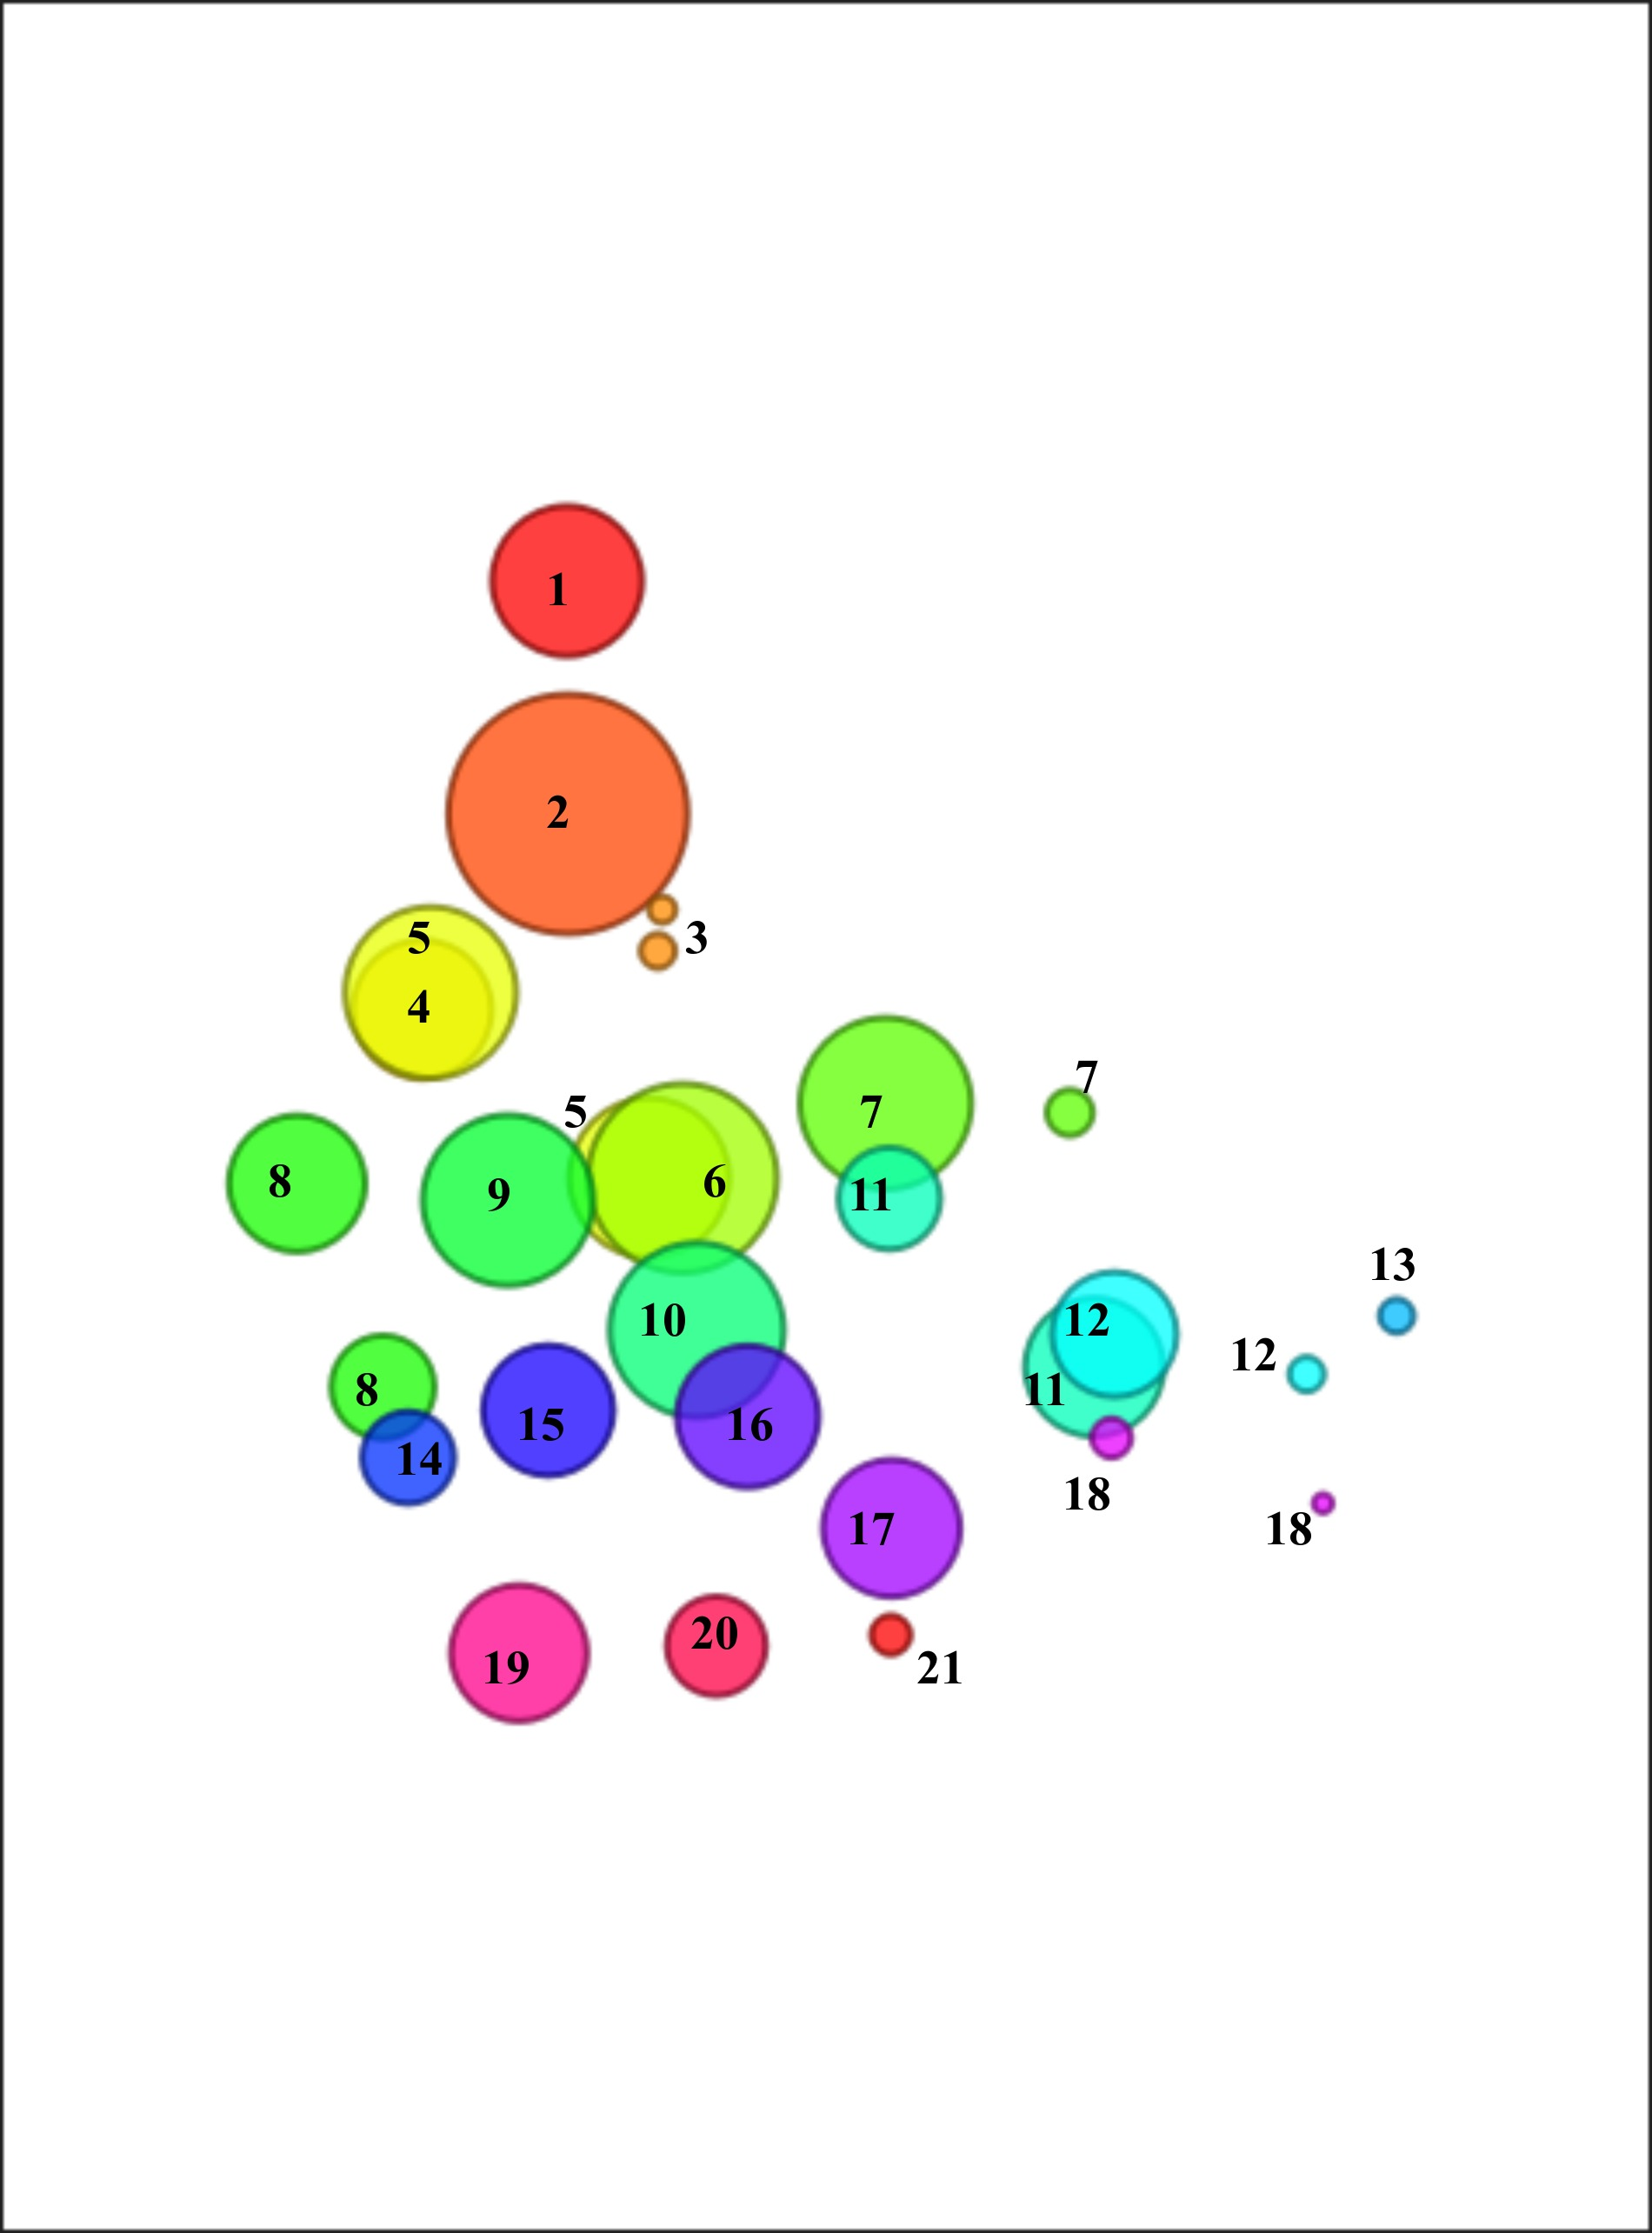
\includegraphics[width=0.6\columnwidth]{figs/engine-block-clusters-tf.jpg}
    \caption{Initial transfer function definition and volume features for the engine block dataset. Selected attributes: \{intensity, skewness, gradient magnitude and variance\} (\(k=4\)). Method parameters: $minPts=4$; $\varepsilon=0.35$ and $\alpha=0.85$.}
    \label{fig:engine-block-clusters-tf}
\end{figure}

\begin{figure}[htb!]
    \centering
    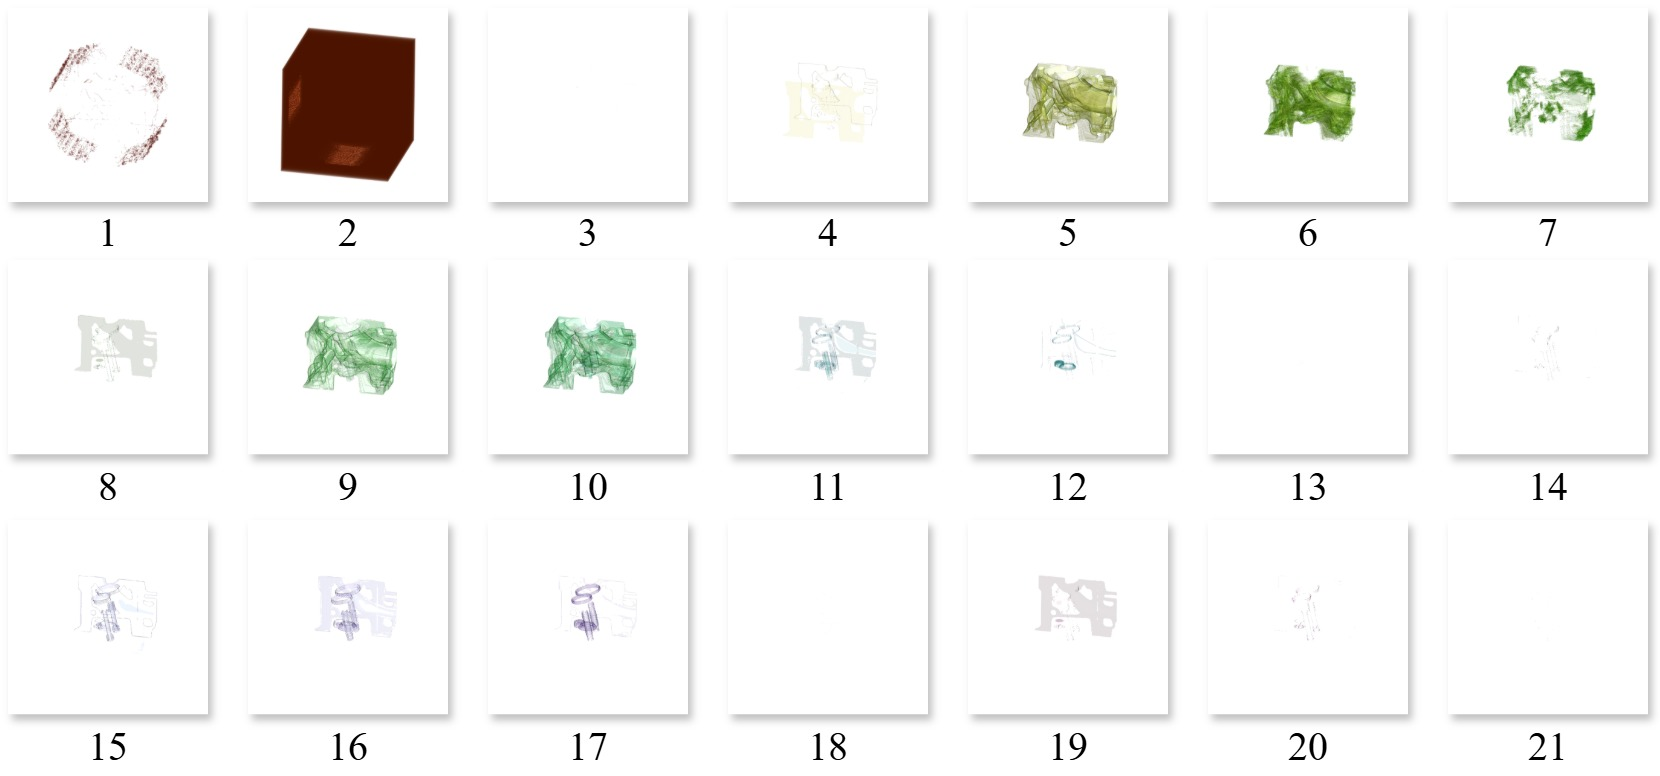
\includegraphics[width=\columnwidth]{figs/engine-block-clusters.jpg}
    \caption{Rendered volume features for the engine block dataset.}
    \label{fig:engine-block-clusters}
\end{figure}

Figure~\ref{fig:engine-block-groups} shows a volume exploration simulation revealing engine components, based on the selected attribute subset.

\begin{figure}[htb!]
    \centering
    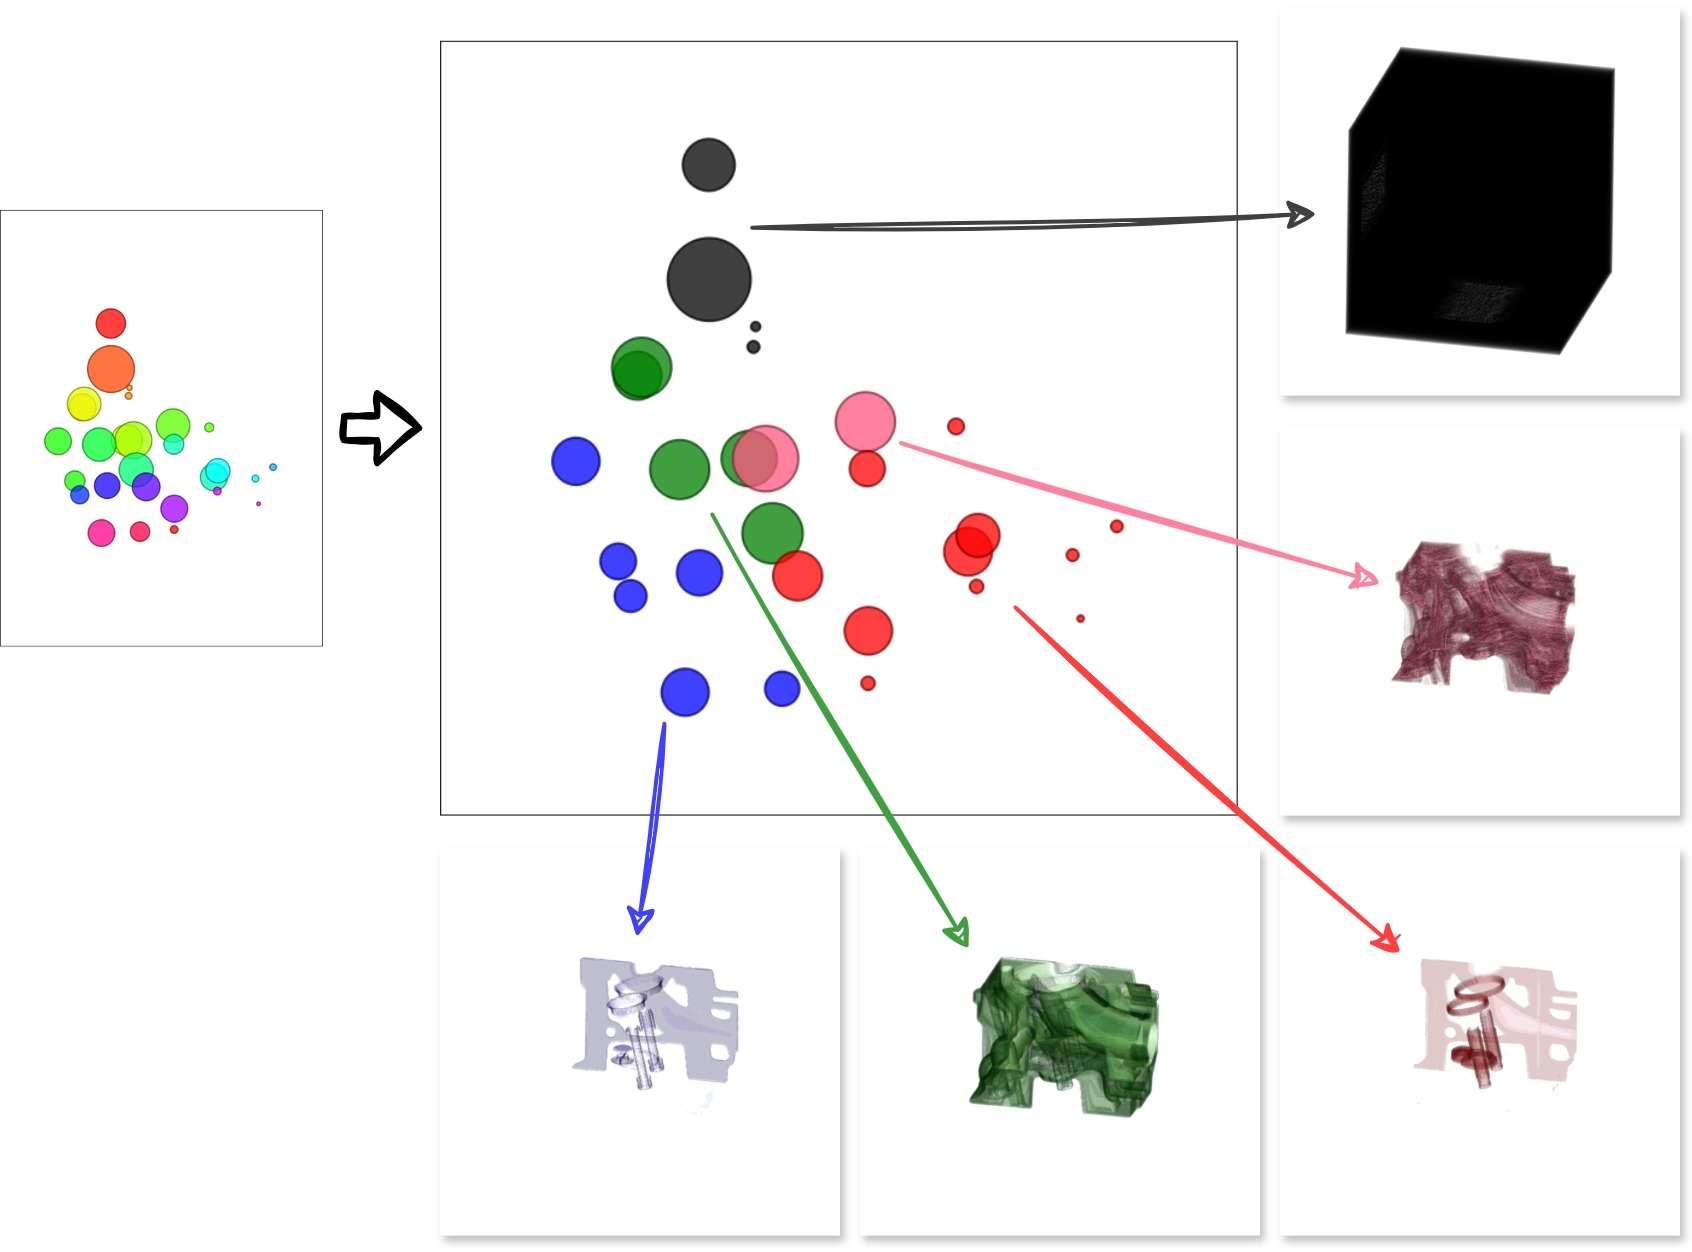
\includegraphics[width=\columnwidth]{figs/engine-block-groups.jpg}
    \caption{User-refined transfer function definition and volume features of interest for block dataset.}
    \label{fig:engine-block-groups}
\end{figure}

\subsubsection{Knees dataset}
\label{subsubsect:knees-dataset}

For the knees dataset, a set of \(k = 5\) attributes was selected: \{intensity, variance, absolute deviation, energy and contrast\}. Preliminary classification is shown in Fig.~\ref{fig:knees-tf-clusters}, with rendered details in Fig.~\ref{fig:knees-clusters}. Method parameters: $minPts=4$, $\varepsilon=0.35$ and $\alpha=0.9$.

\begin{figure}[htb!]
    \centering
    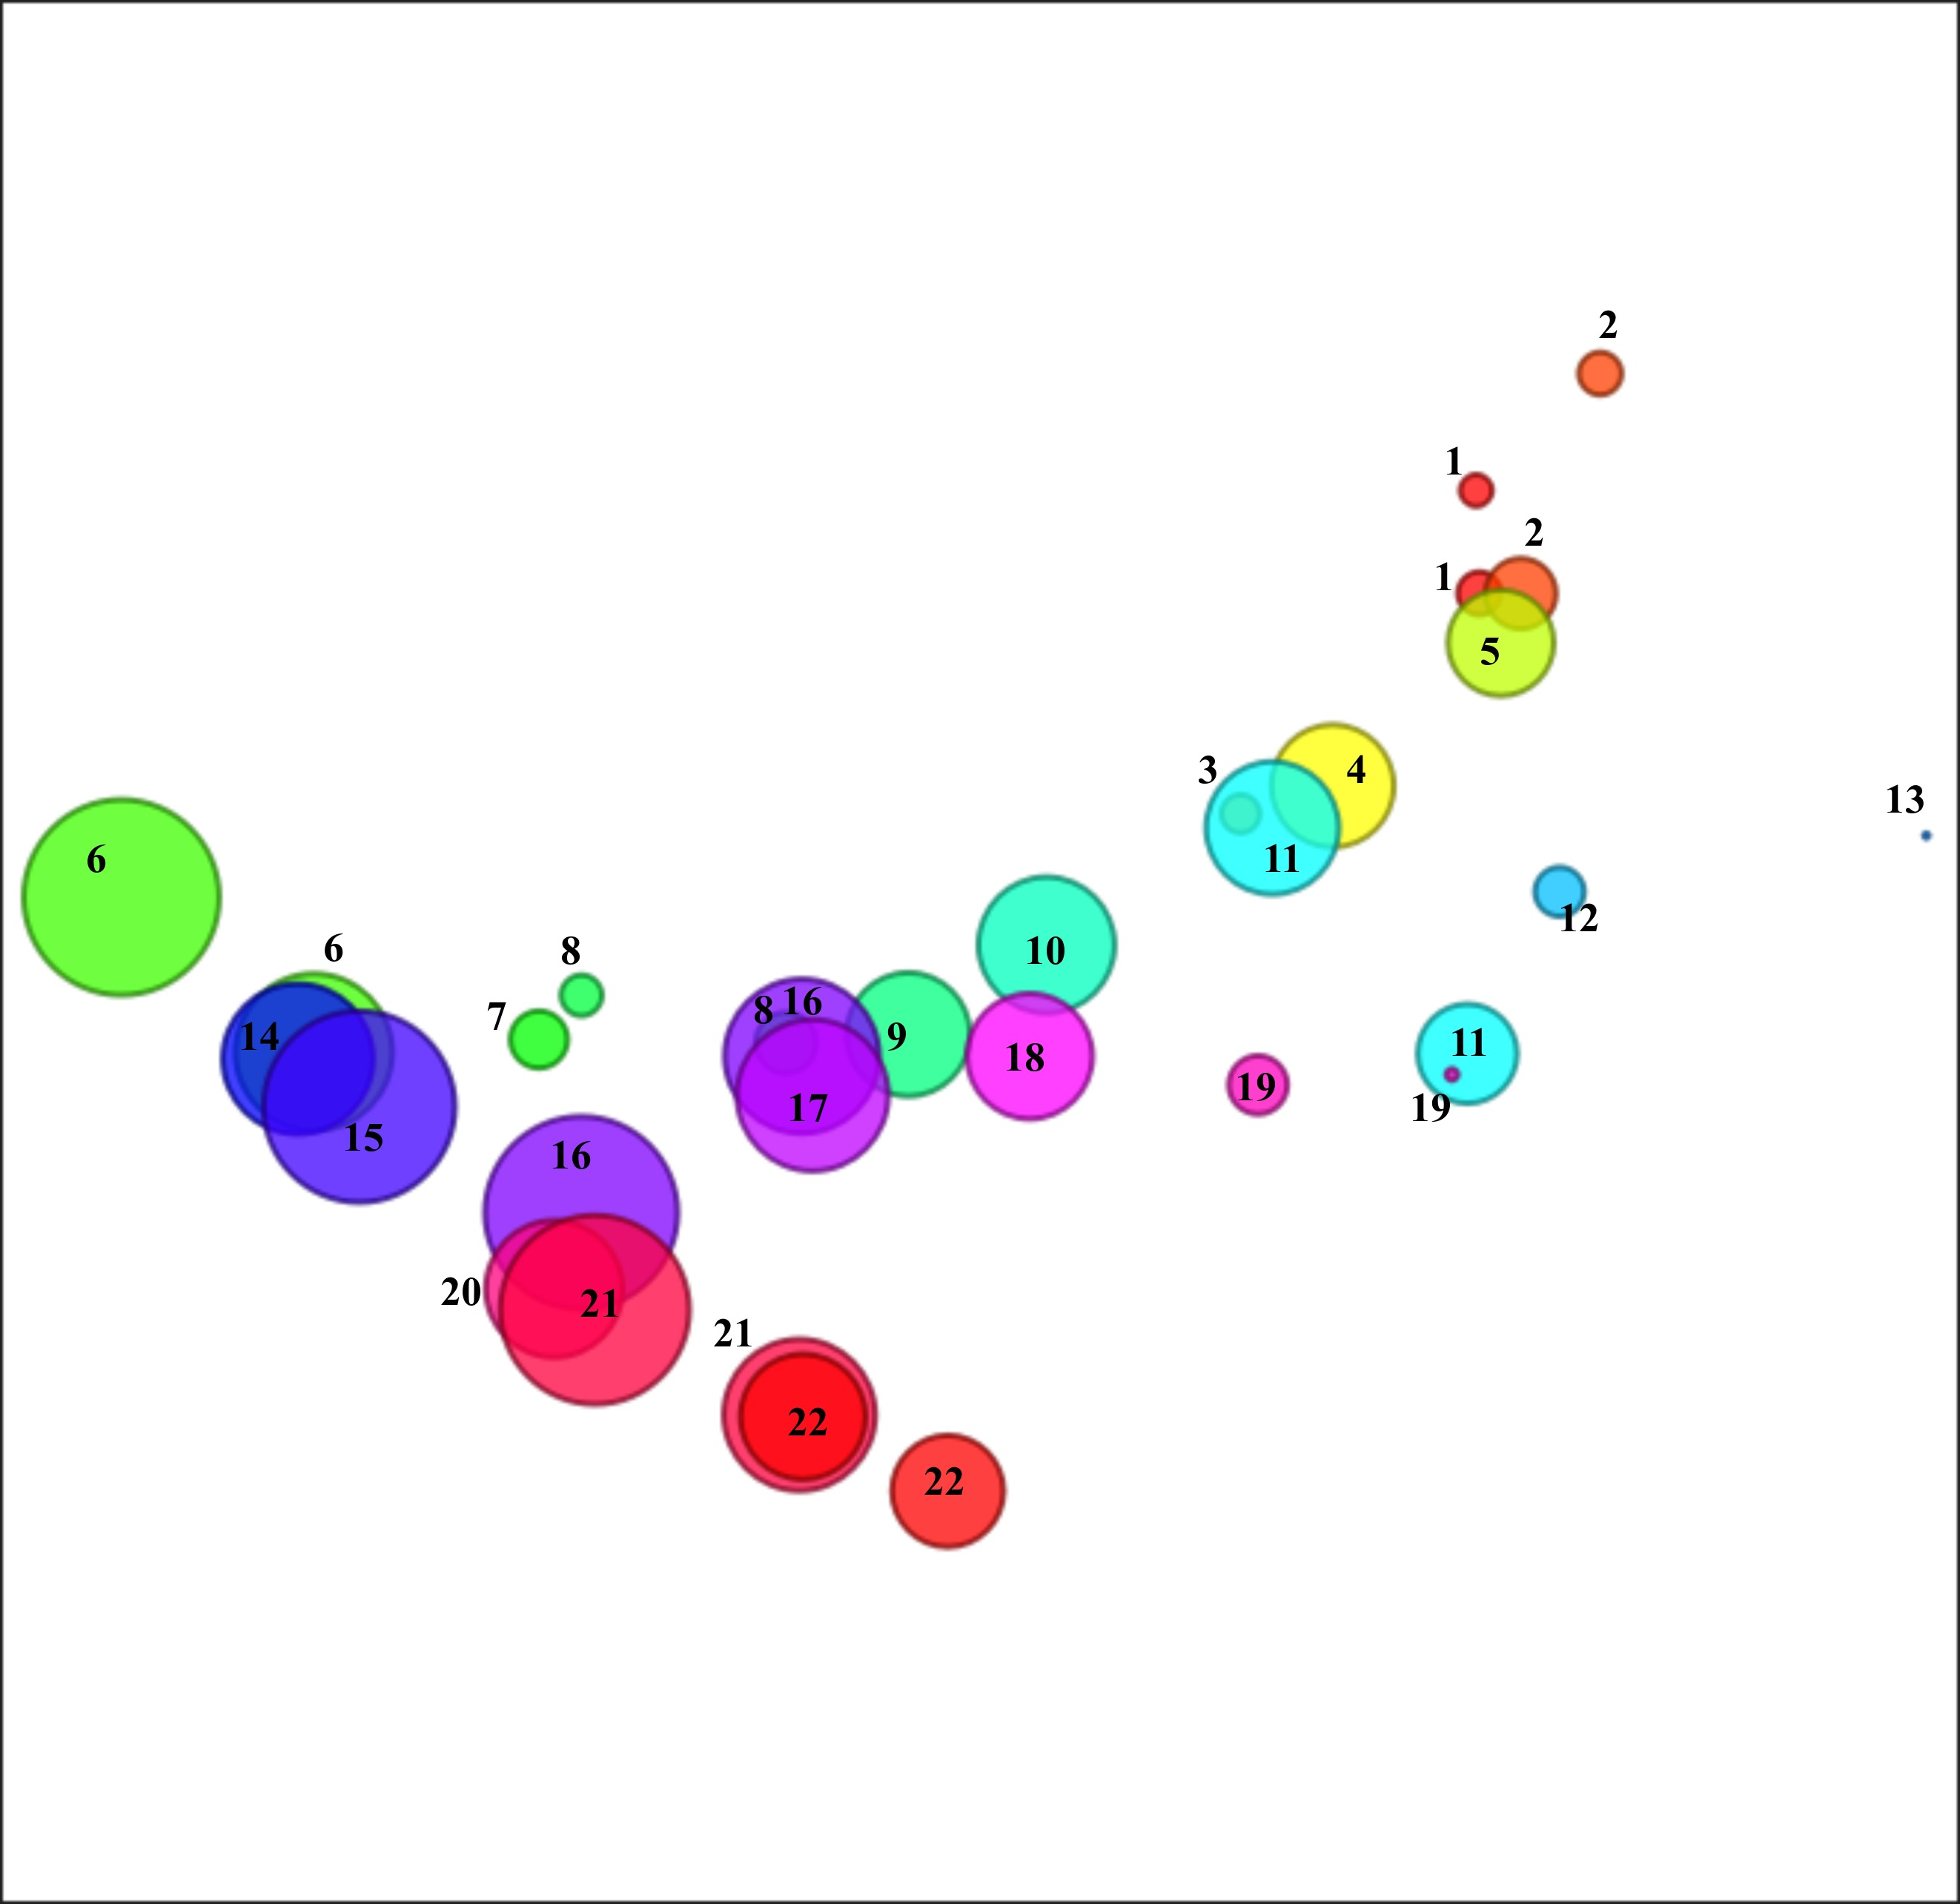
\includegraphics[width=0.7\columnwidth]{figs/knees-clusters-tf.jpg} 
    \caption{Initial transfer function definition and volume features for the knees dataset. Selected attributes: \{intensity, variance, absolute deviation, energy, contrast\} (\(k=5\)). Method parameters: $minPts=4$, $\varepsilon=0.35$ and $\alpha=0.9$.}
    \label{fig:knees-tf-clusters}
\end{figure}

\begin{figure}[htb!]
    \centering
    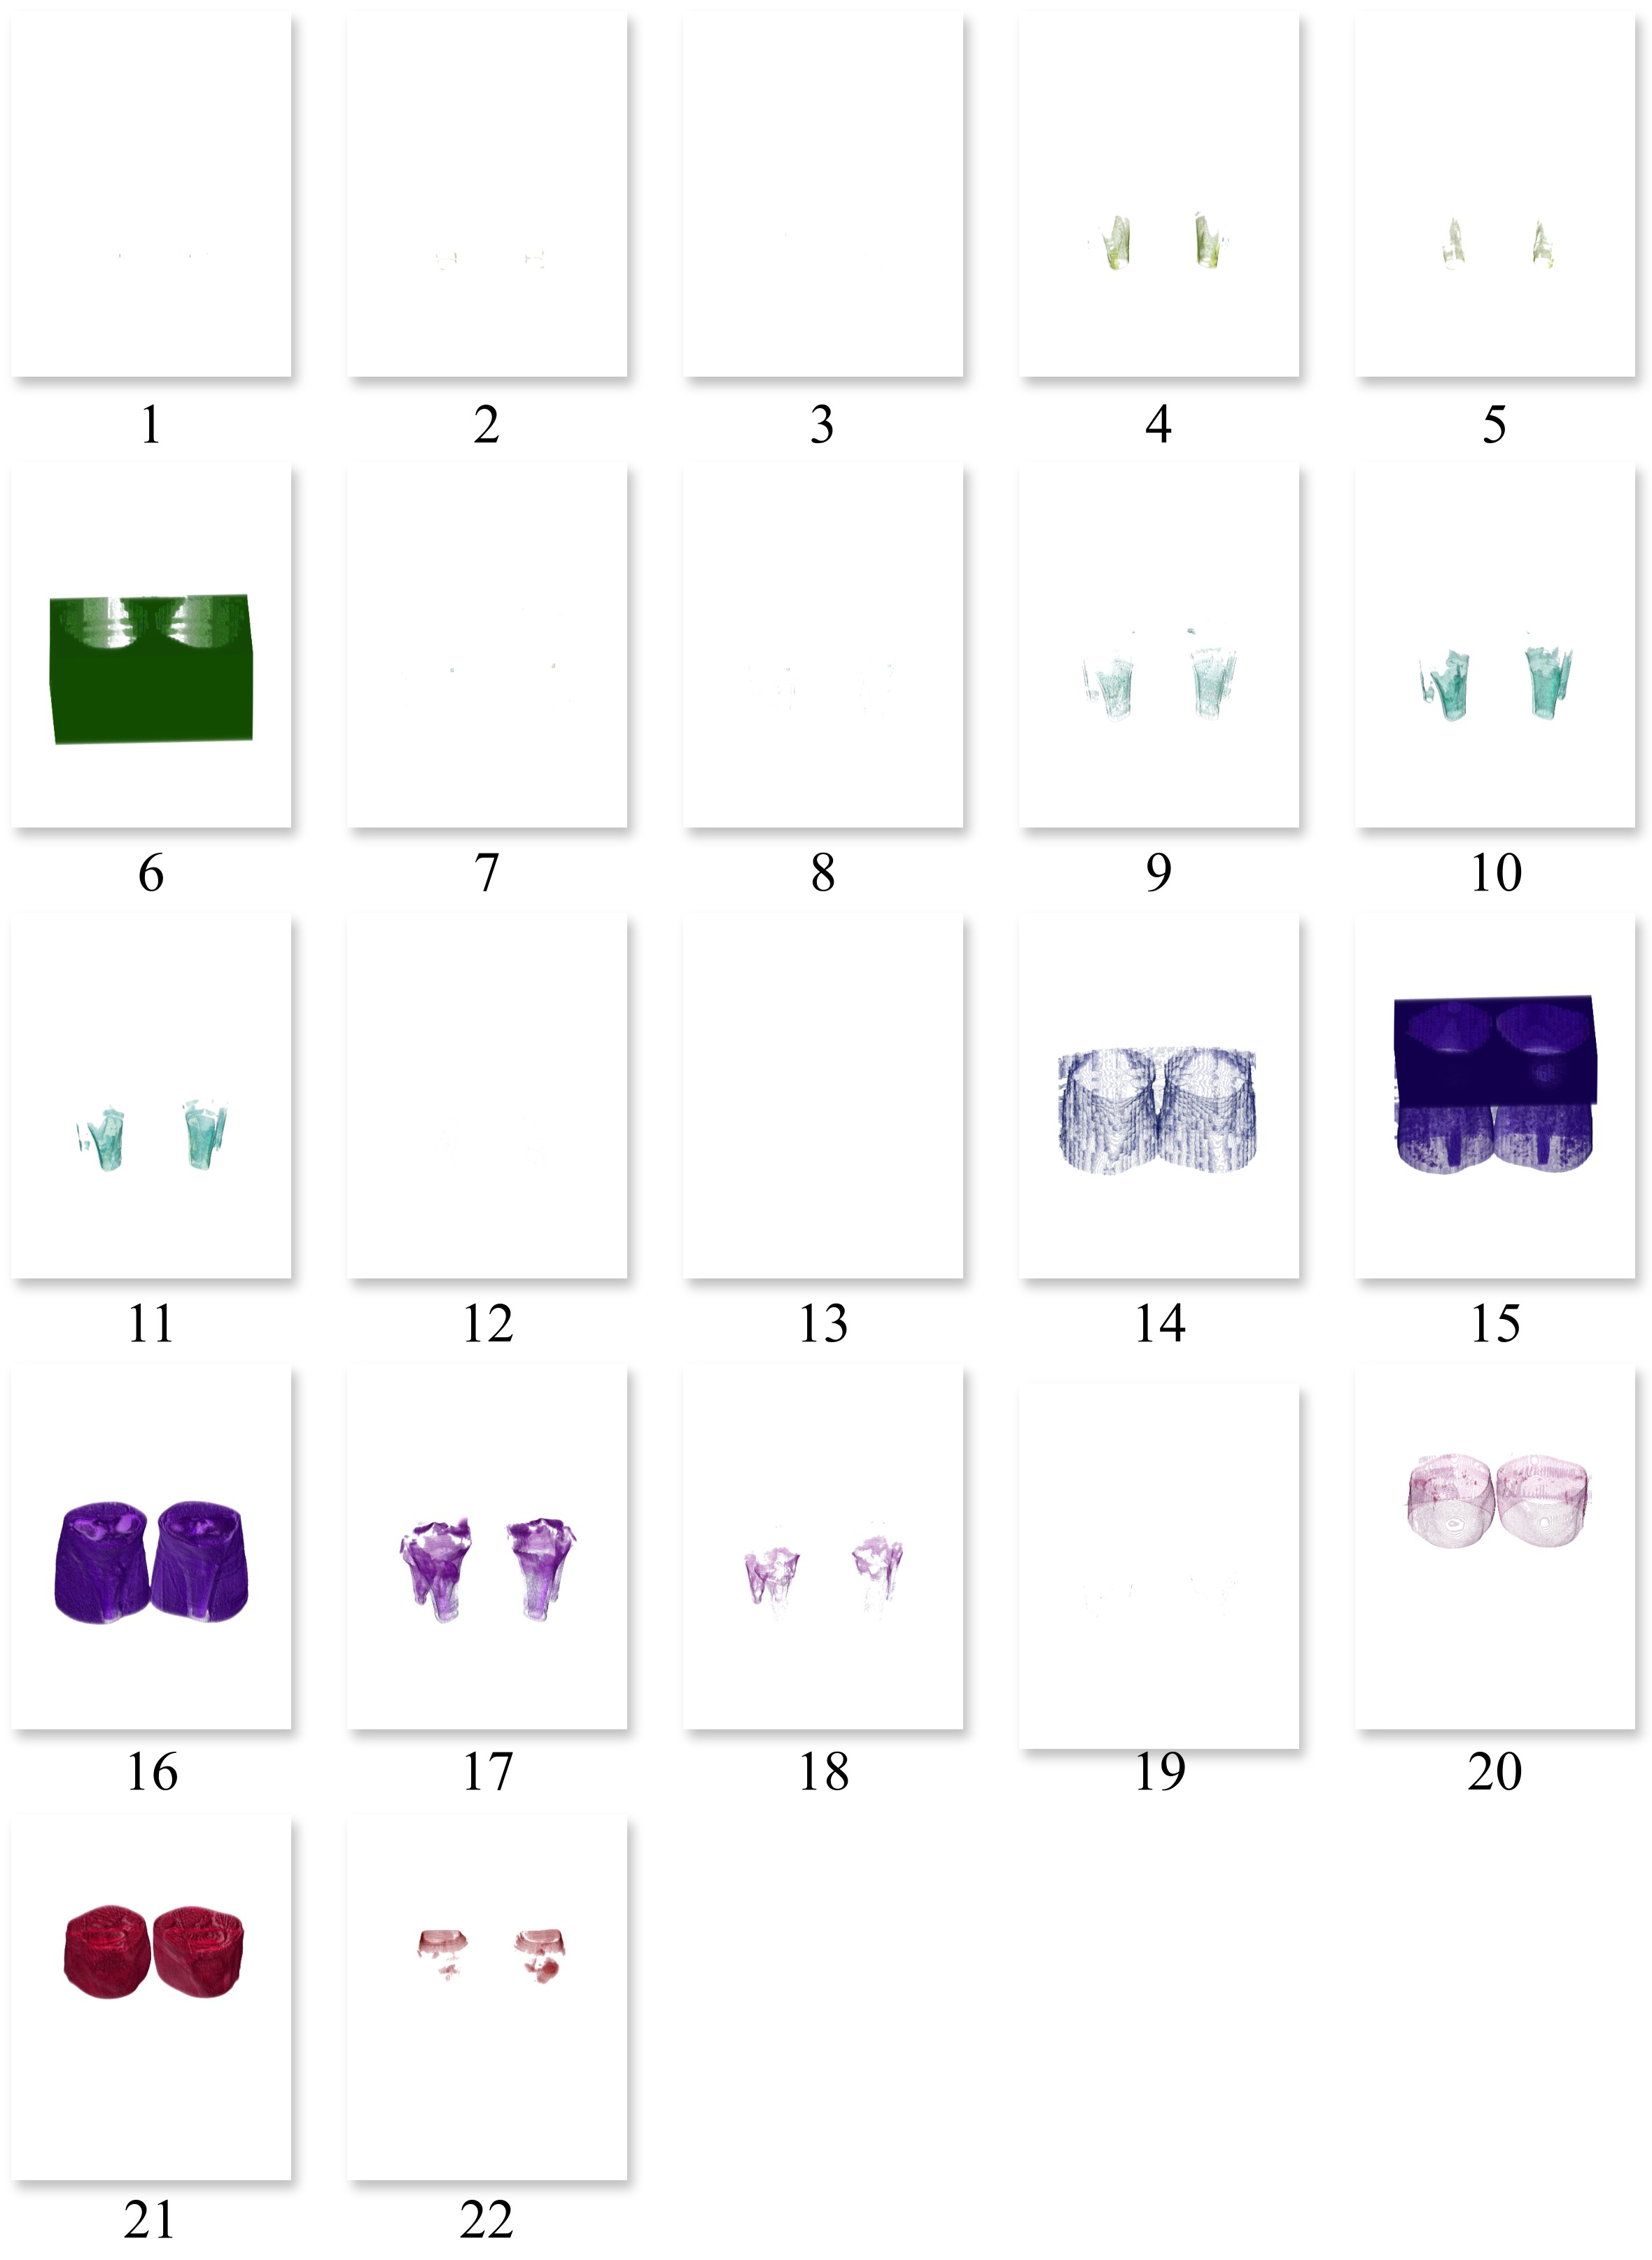
\includegraphics[width=\columnwidth]{figs/knees-clusters.jpg} 
    \caption{Rendered volume features for the knees dataset.}
    \label{fig:knees-clusters}
\end{figure}

Figure~\ref{fig:knees-groups} illustrates the empirically grouped bones and muscles: femur, tibia, patella, fibula, thigh and knee muscles.

\begin{figure}[htb!]
    \centering
    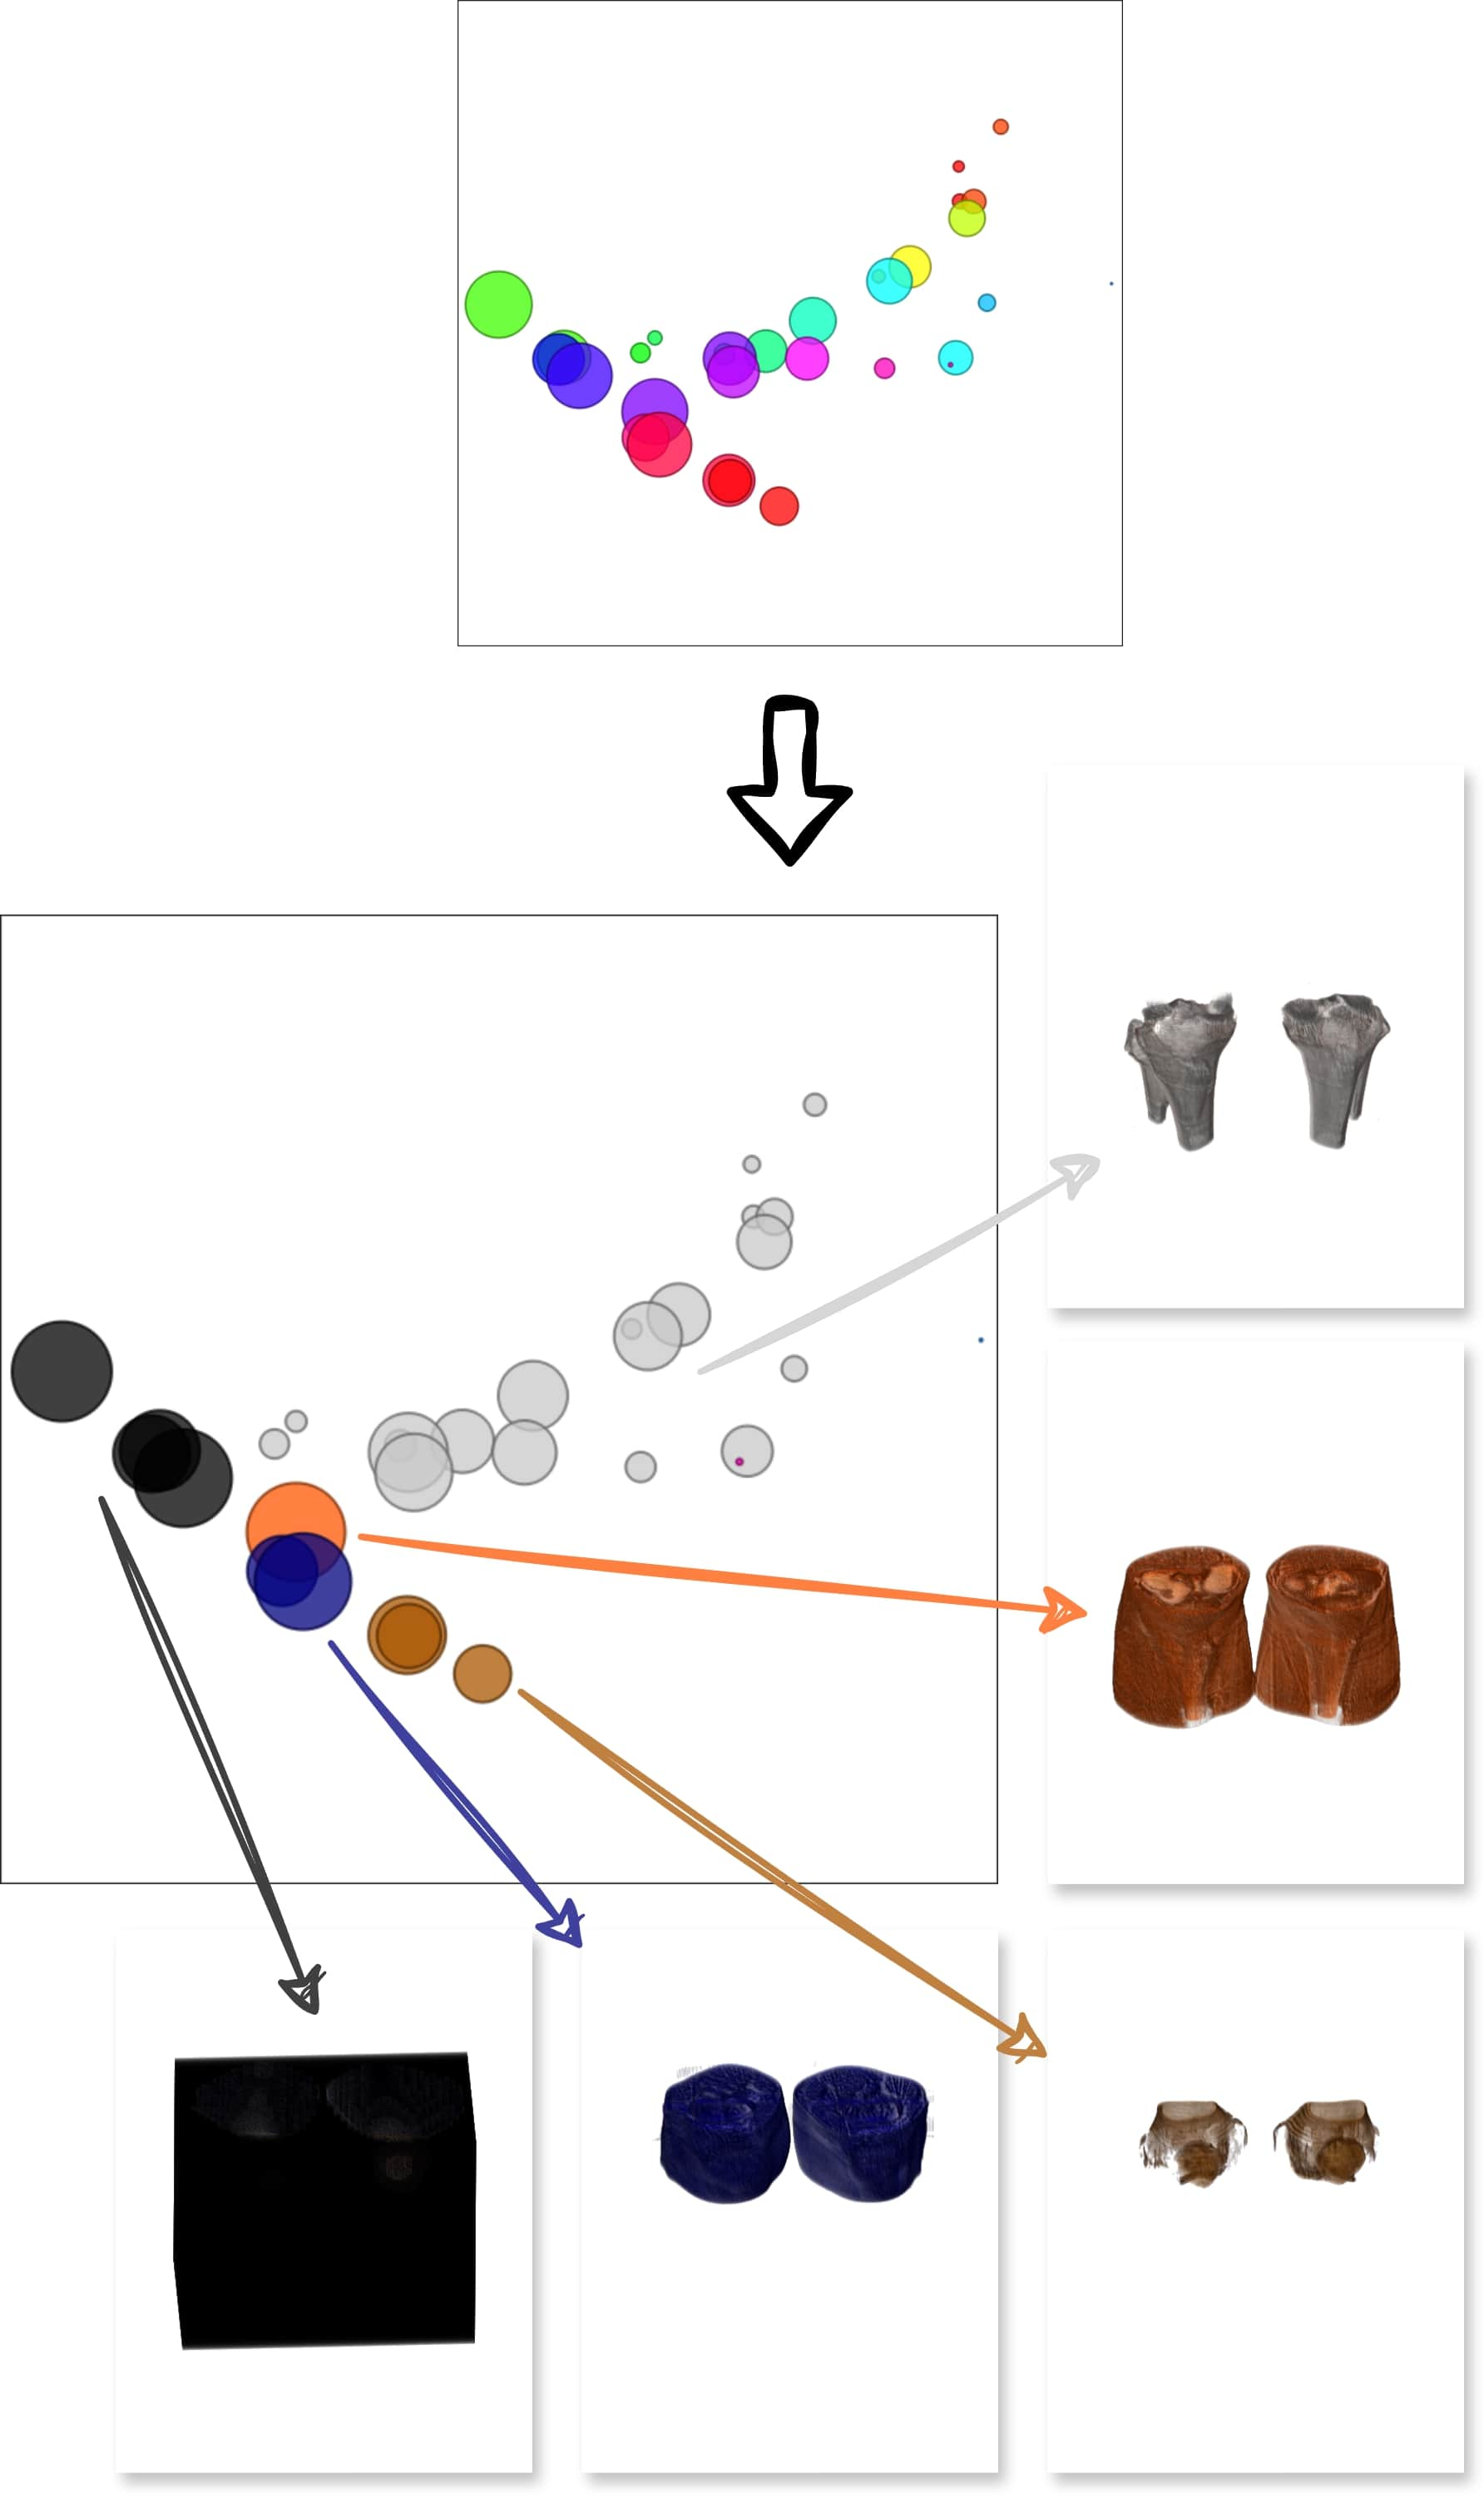
\includegraphics[width=\columnwidth]{figs/knees-groups.jpg}
    \caption{User-refined transfer function definition and volume features of interest for knees dataset.}
    \label{fig:knees-groups}
\end{figure}

\subsubsection{Tooth dataset}
\label{subsubsect:tooth-dataset}

For the tooth dataset, a set of \(k = 6\) attributes was selected: \{intensity, variance, absolute deviation, energy, contrast and entropy\}. Figure~\ref{fig:tooth-clusters-tf} shows the volume exploration space, with rendered details in Fig.~\ref{fig:tooth-clusters}. Method parameters: $minPts=4$, $\varepsilon=0.23$ and $\alpha=0.9$.

\begin{figure}[htb!]
    \centering
    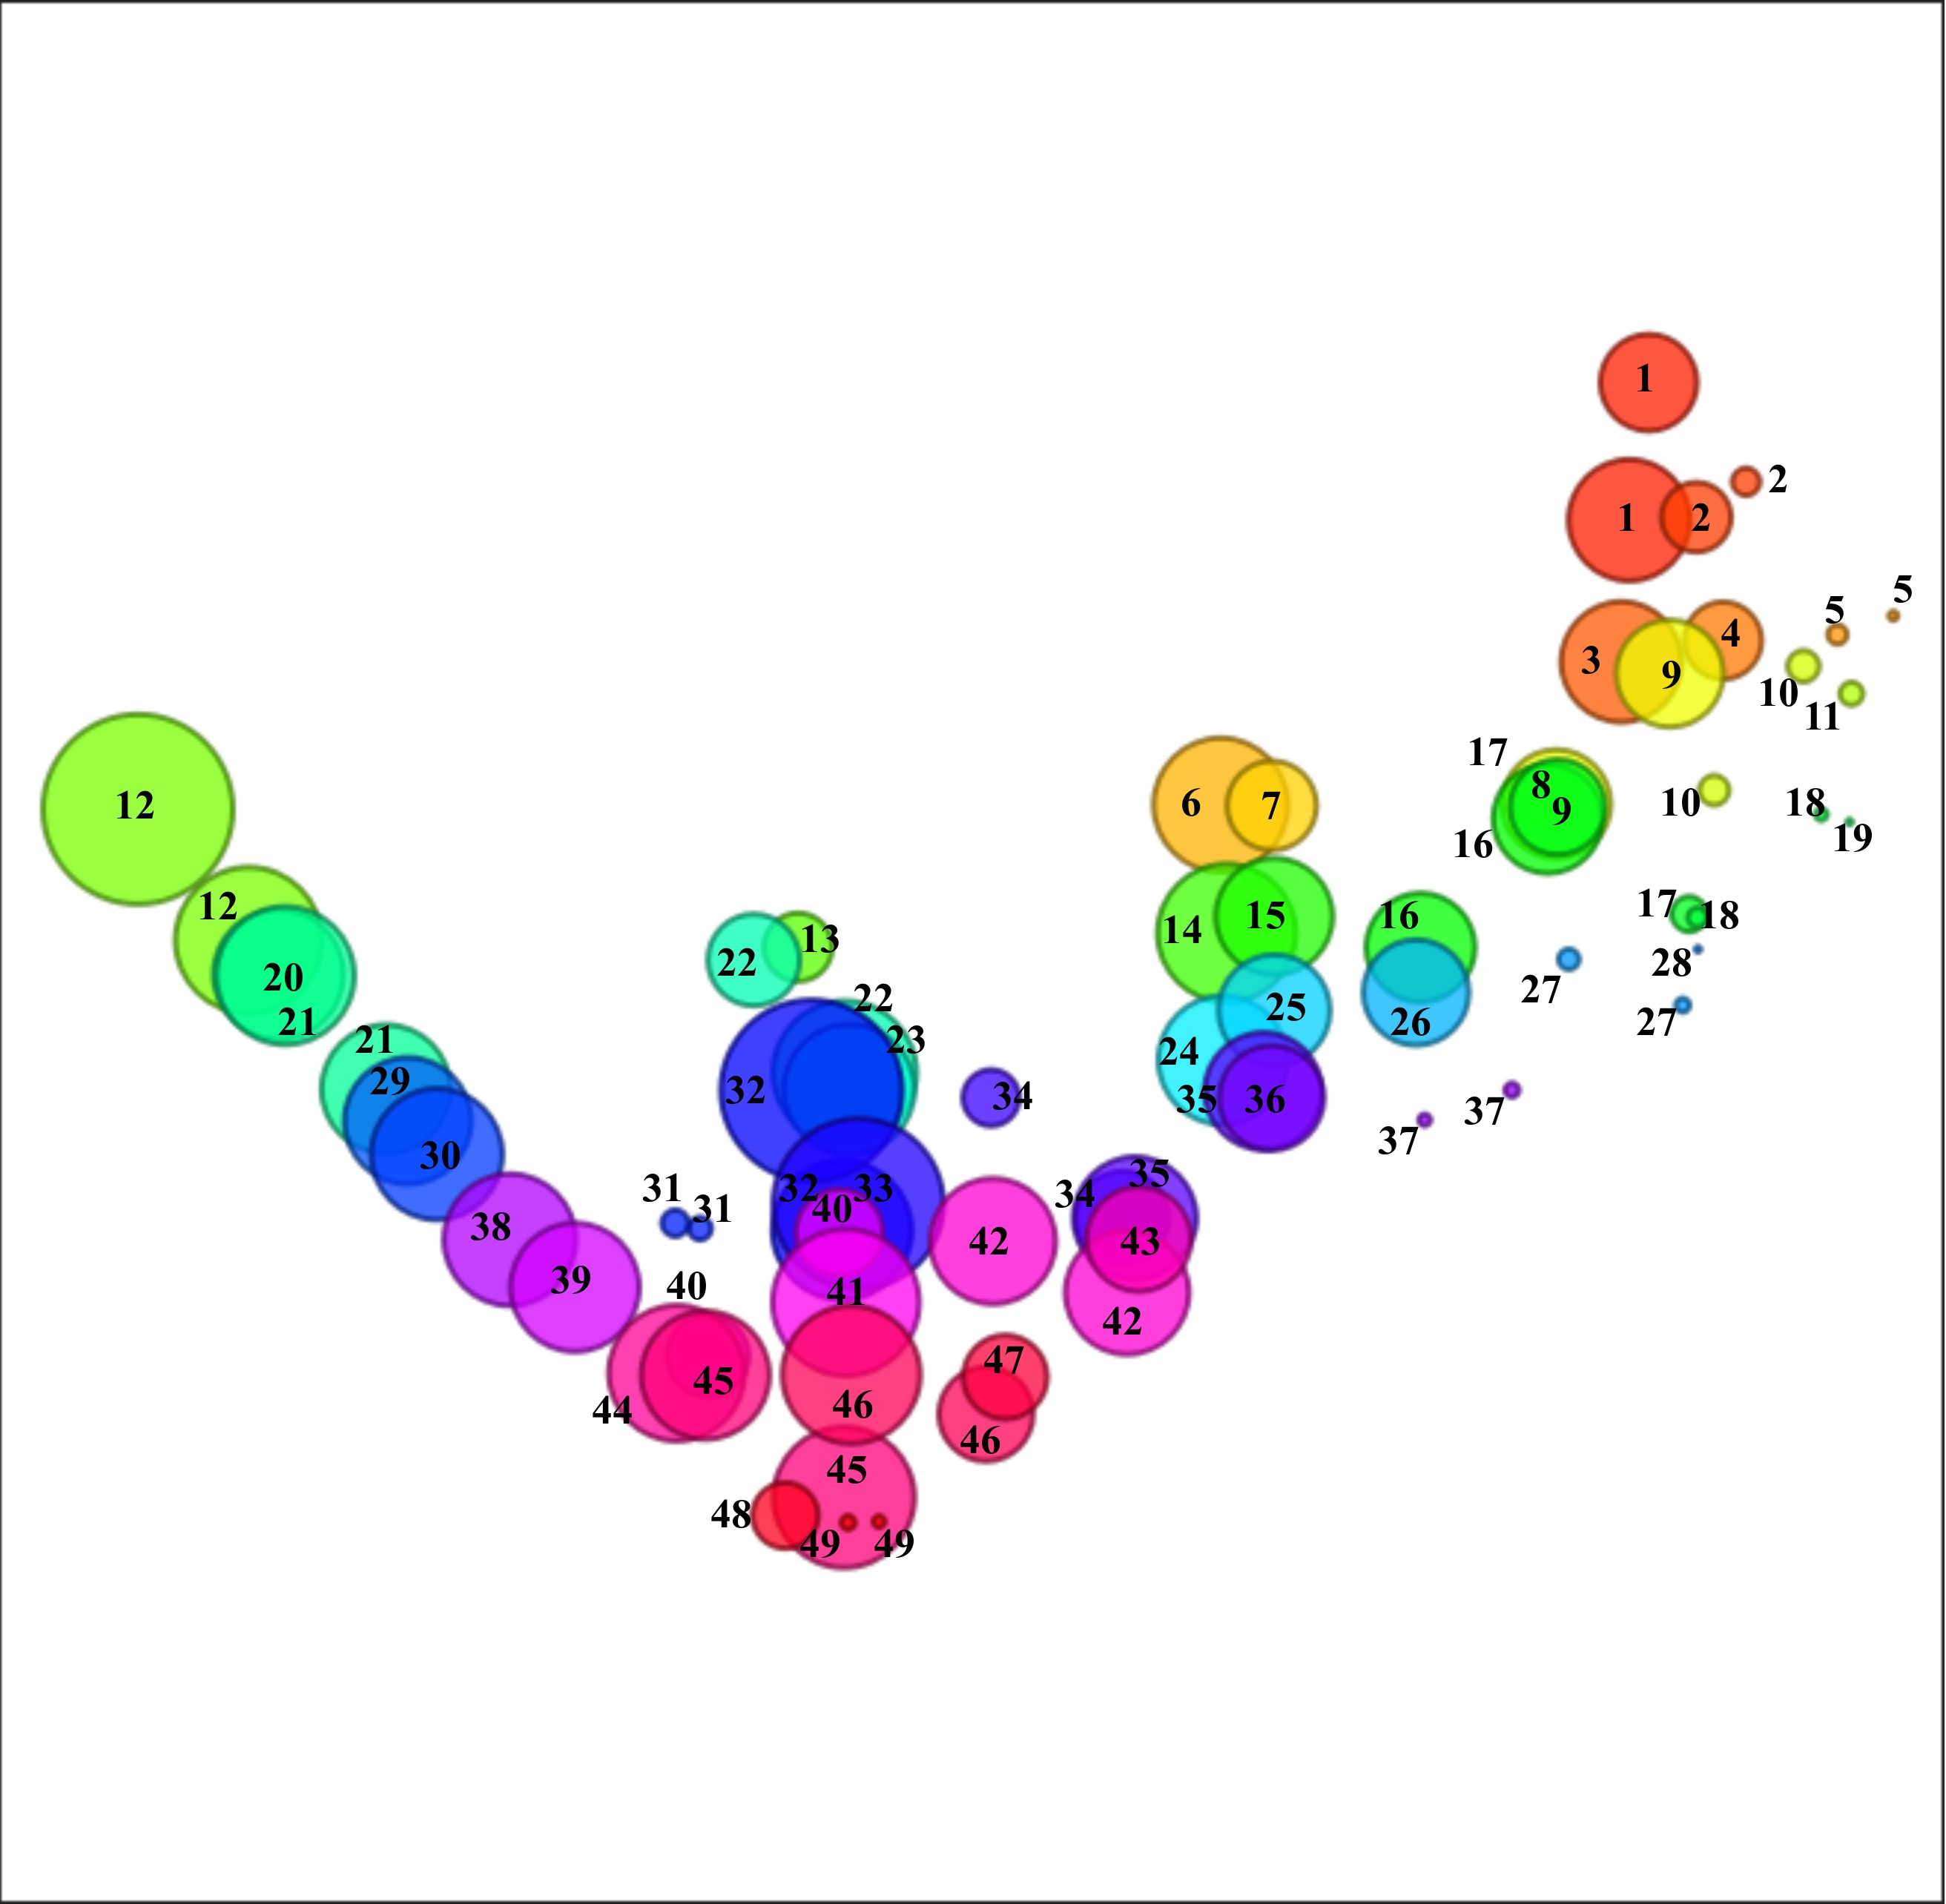
\includegraphics[width=0.7\columnwidth]{figs/tooth-clusters-tf.jpg} 
    \caption{Initial transfer function definition and volume features for the tooth dataset. Selected attributes: \{intensity, variance, absolute deviation, energy, contrast and entropy\} (\(k=6\)). Method parameters: $minPts=4$; $\varepsilon=0.23$; $\alpha=0.9$.}
    \label{fig:tooth-clusters-tf}
\end{figure}

\begin{figure}[htb!]
    \centering
    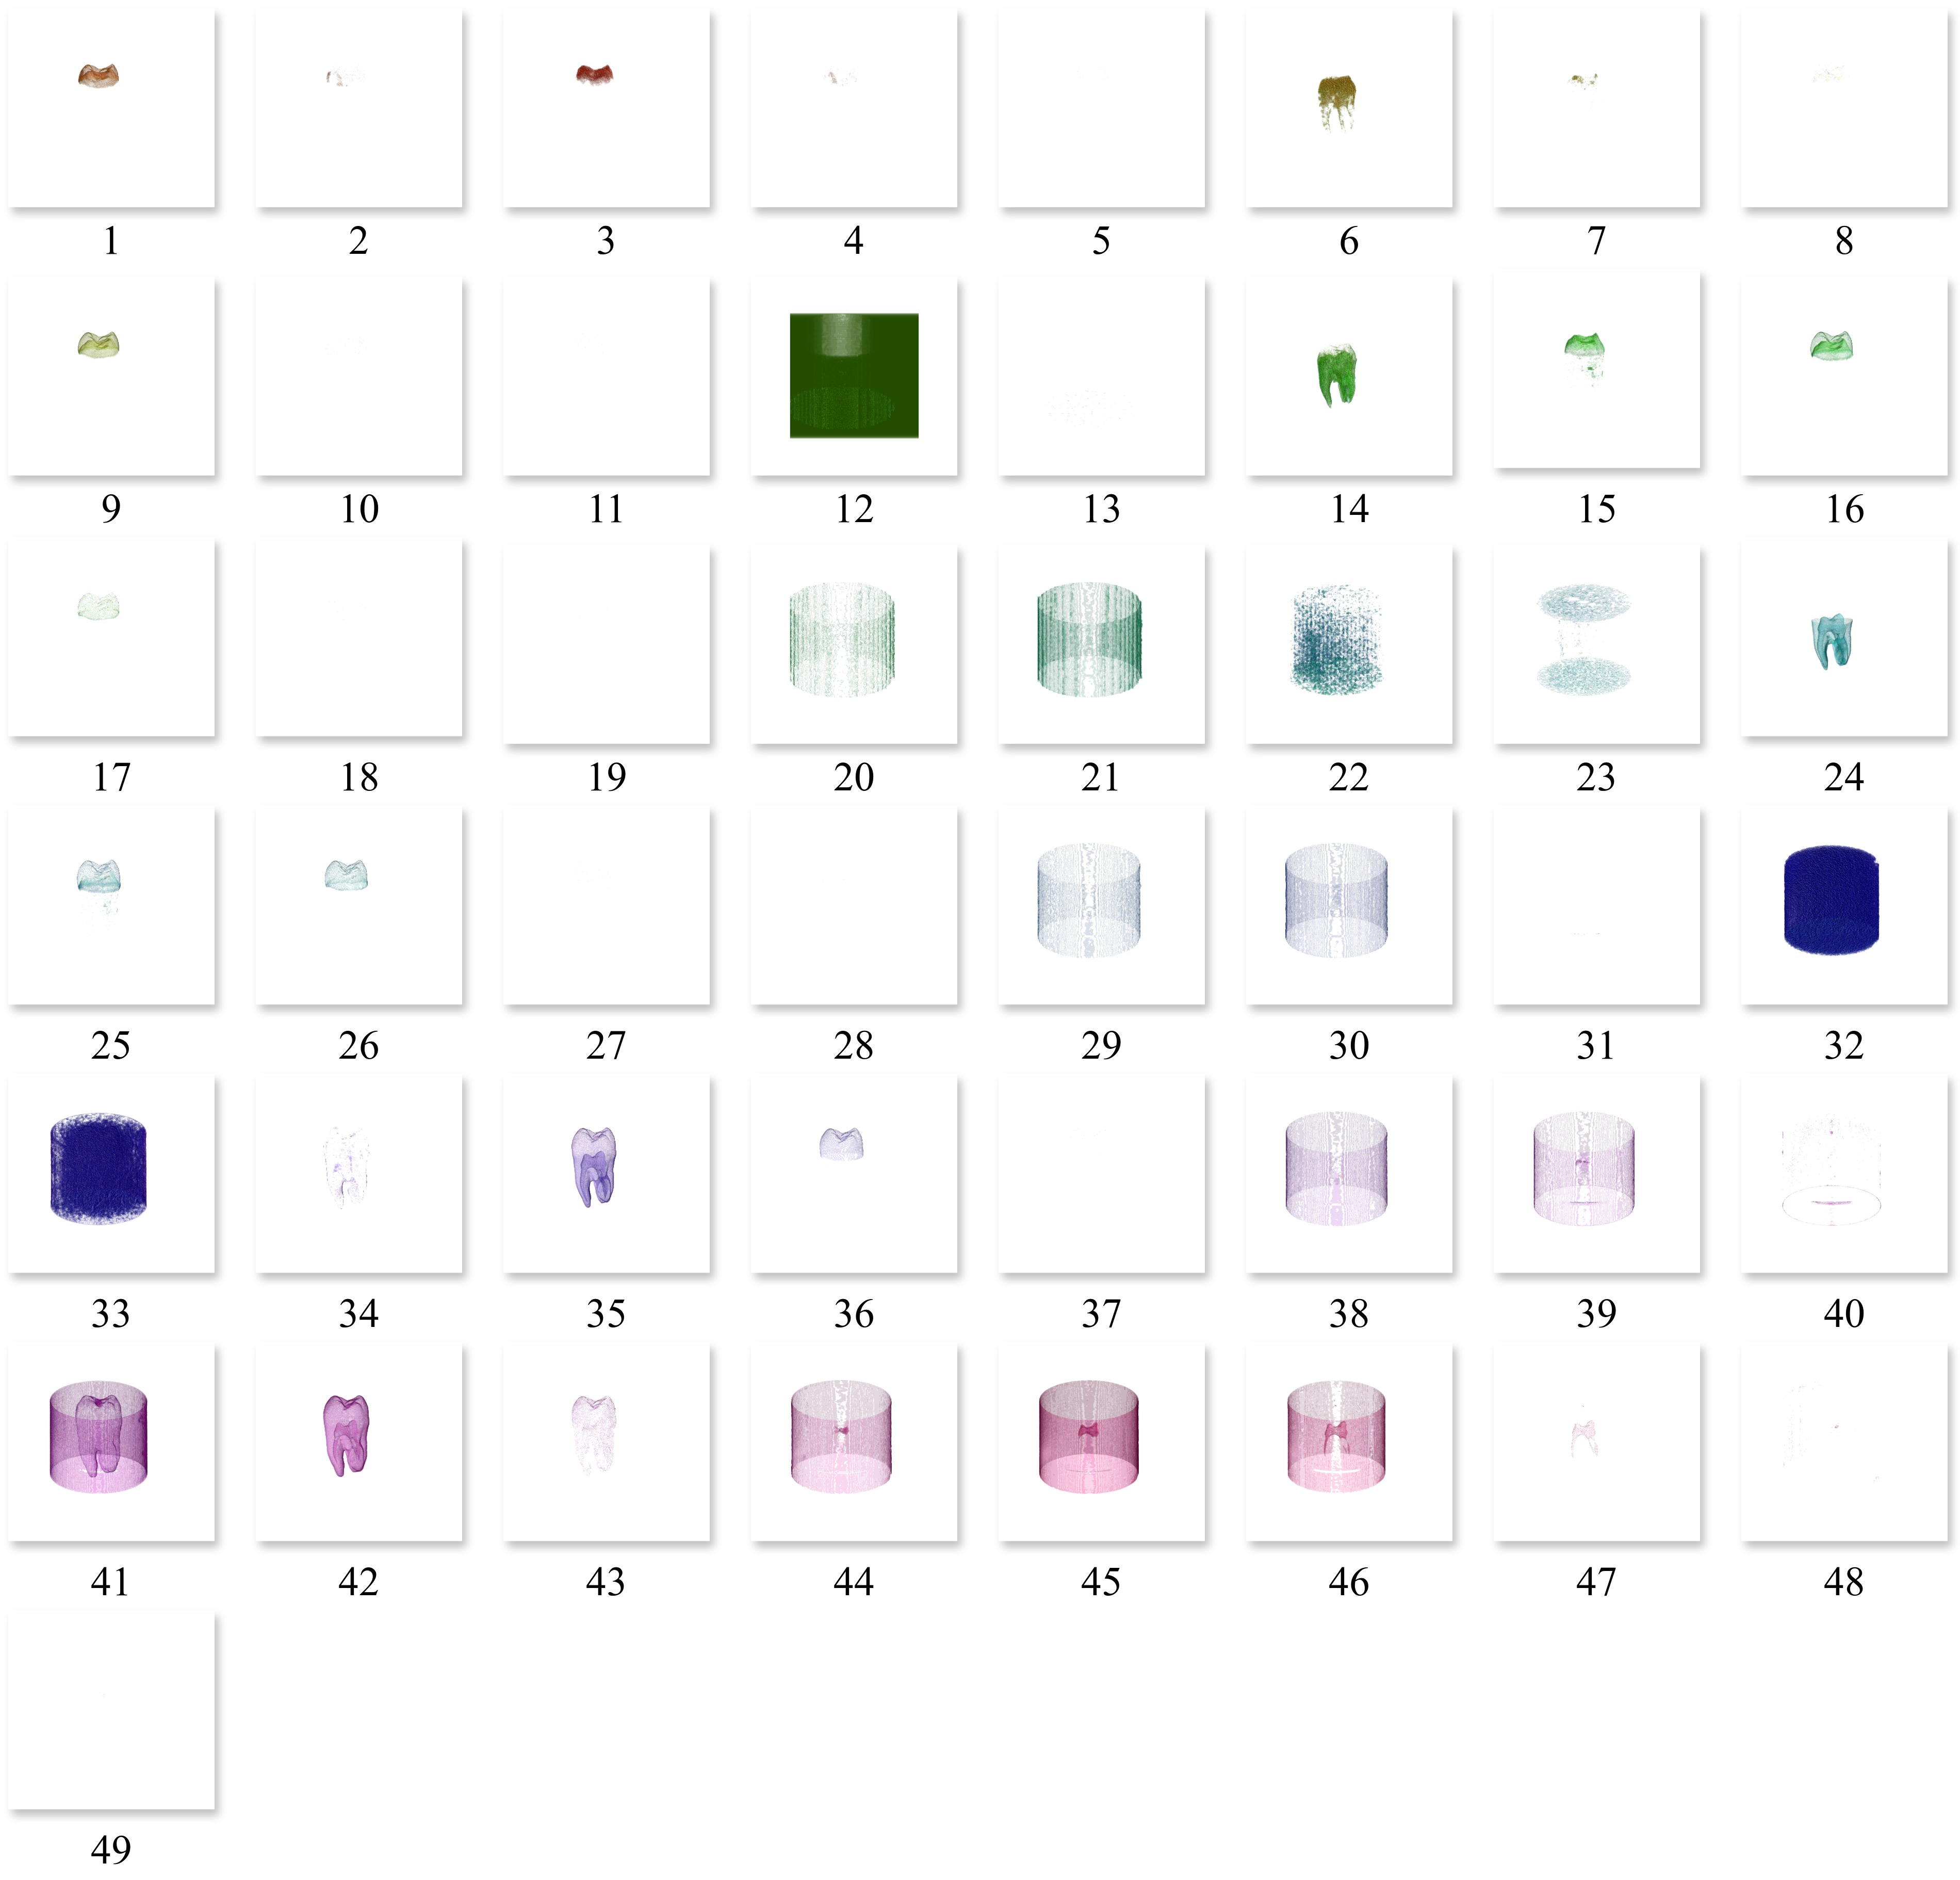
\includegraphics[width=\columnwidth]{figs/tooth-clusters.jpg} 
    \caption{Rendered volume features for the tooth dataset.}
    \label{fig:tooth-clusters}
\end{figure}

Figure~\ref{fig:tooth-groups} shows empirically grouped tooth structures: enamel, pulp, dentin, crown, entire tooth and immersion fluid.

\begin{figure}[htb!]
    \centering
    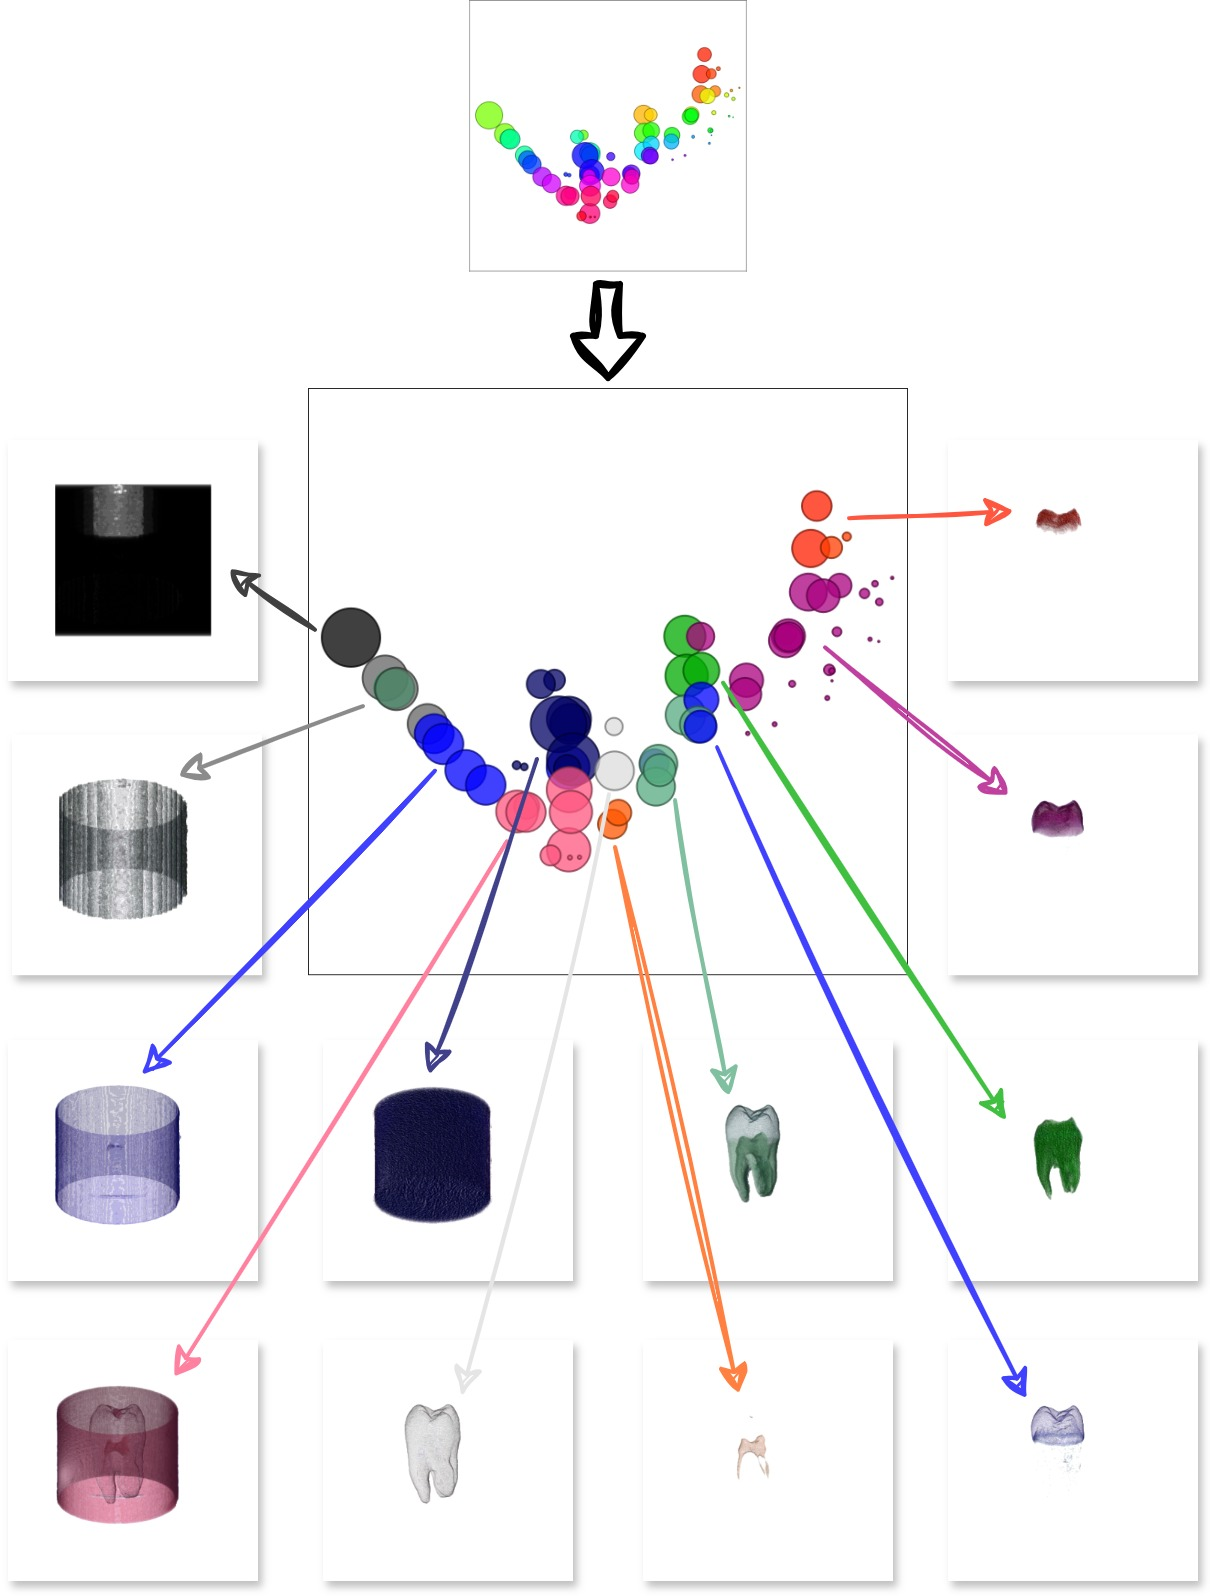
\includegraphics[width=0.8\columnwidth]{figs/tooth-groups.jpg}
    \caption{User-refined transfer function definition and volume features of interest for tooth dataset.}
    \label{fig:tooth-groups}
\end{figure}


\subsection{Runtime}
\label{subsect:runtime-analysis}

Table~\ref{tab:runtime-analysis} presents the runtimes (in seconds) for each dataset.

\begin{table}[!htbp]
\caption{Runtime (seconds) of the proposed method per dataset.}
\label{tab:runtime-analysis}
\centering
    \begin{tabular}{@{}>{\centering\arraybackslash}m{0.4\columnwidth}>{\centering\arraybackslash}m{0.15\columnwidth}>{\centering\arraybackslash}m{0.15\columnwidth}>{\centering\arraybackslash}m{0.15\columnwidth}@{}}
        \toprule
            & \textbf{Engine block} & \textbf{Knees} & \textbf{Tooth} \\
        \midrule
        \textbf{Dimensionality reduction} & 7.50 & 7.98 & 36.05 \\
        \textbf{Clustering} & 51.52 & 102.77 & 19.42 \\
        \textbf{Representative selection} & 2.23 & 3.15 & 1.33 \\
        \midrule
        \textbf{Transfer function design interface} & 1.48 & 1.86 & 0.79 \\
        \bottomrule
    \end{tabular}
\end{table}

Dimensionality reduction and clustering are the most time-consuming steps. The reduction time depends on dataset size and dimensionality, while clustering, representative selection and TF interface construction operate in 2D and depend mainly on the number of voxels.


Overall, the method incurs minimal time overhead, demonstrating efficient performance and promising scalability for large volume datasets.

\subsection{Parameter choice}
\label{subsect:parameter-choice}

The choice of DBSCAN parameters strongly affects classification outcomes. The $minPts$ parameter can reliably use a default value of 4~\cite{ester1996}, given that FastMap reduces the data to a 2D space. However, the $\varepsilon$ parameter requires careful tuning: larger values produce fewer but larger clusters, while smaller values result in more numerous, smaller clusters.

The SSS distance factor ($\alpha$) similarly influences clustering granularity, varying inversely with the number of pivots selected per cluster.

